\chapter{Results}\label{cha:results}

\section{Depth and ego motion}

\begin{table}[H]
\begin{tabular}{|l|c|c|c|c|c|c|c|c|c|c|}
\hline
 & Net & DS & W & Edge & Norm & Expl & Stat & SSIM & Comb & US \\
\hline
C1 & SL & K & di &  &  & $ \times $ &  &  & avg &  \\
\hline
C2 & SL & K & de &  &  & $ \times $ &  &  & avg &  \\
\hline
C3 & SL & K & de &  &  &  &  &  & avg &  \\
\hline
C4 & SL & K & de &  &  &  & $ \times $ &  & avg &  \\
\hline
C5 & SL & K & de & $ \times $ &  &  & $ \times $ &  & avg &  \\
\hline
C6 & SL & K & de & $ \times $ &  &  & $ \times $ & $ \times $ & min &  \\
\hline
C7 & SL & K & de & $ \times $ & $ \times $ &  & $ \times $ & $ \times $ & min &  \\
\hline
C8 & SL & K & de & $ \times $ & $ \times $ &  & $ \times $ & $ \times $ & min & $ \times $ \\
\hline
C9 & SL & L & de & $ \times $ & $ \times $ &  & $ \times $ & $ \times $ & min & $ \times $ \\
\hline
C10 & M2 & K & de &  &  &  & $ \times $ &  & avg &  \\
\hline
C11 & M2 & K & de & $ \times $ & $ \times $ &  & $ \times $ & $ \times $ & min &  \\
\hline
C12 & M2 & K & de & $ \times $ & $ \times $ &  & $ \times $ & $ \times $ & min & $ \times $ \\
\hline
C13 & M2 & L & de & $ \times $ & $ \times $ &  & $ \times $ & $ \times $ & min & $ \times $ \\
\hline
\end{tabular}
\caption{Different configurations of network architecutes, training datasets and loss terms evaluated to find the best performance}
\label{table:configurations}
\end{table}


\begin{table}[H]
{\setlength{\tabcolsep}{0.4em}
\begin{tabular}{|r|r|c||l|l|l|l||l|l|l||l|}
\hline
E & C & DS & AbsRel & SqRel & RMSE & RMSLE & $1.25$ & $1.25^2$ & $1.25^3$ & Ego \\
\hline
1 & 1 & K & 0.362 & 13.469 & 8.759 & 0.372 & 0.730 & 0.884 & 0.933 & 0.020 \\
\hline
2 & 2 & K & 0.184 & 1.718 & 4.953 & 0.258 & 0.776 & 0.915 & 0.960 & 0.020 \\
\hline
3 & 3 & K & 0.174 & 1.405 & 4.829 & 0.249 & 0.784 & 0.920 & 0.964 & 0.024 \\
\hline
4 & 4 & K & 0.140 & 0.793 & 4.549 & 0.217 & 0.818 & 0.939 & 0.976 & 0.020 \\
\hline
5 & 5 & K & 0.143 & 0.819 & 4.708 & 0.222 & 0.810 & 0.937 & 0.975 & 0.022 \\
\hline
6 & 6 & K & 0.133 & 0.727 & 4.305 & 0.204 & 0.843 & 0.950 & 0.979 & 0.023 \\
\hline
7 & 7 & K & 0.137 & 0.797 & 4.282 & 0.208 & 0.837 & 0.948 & 0.977 & 0.024 \\
\hline
8 & 8 & K & 0.135 & 0.778 & 4.248 & 0.208 & 0.841 & 0.948 & 0.997 & 0.020 \\
\hline
9 & 8 & L & 0.340 & 7.811 & 23.071 & 0.447 & 0.457 & 0.734 & 0.868 & 0.043 \\
\hline
10 & 9 & K & 0.512 & 5.185 & 10.757 & 0.611 & 0.305 & 0.549 & 0.732 & 0.495 \\
\hline
11 & 9 & L & 0.739 & 20.236 & 31.859 & 0.773 & 0.240 & 0.434 & 0.587 & 1.324 \\
\hline
12 & 10 & K & 0.125 & 0.697 & 4.298 & 0.203 & 0.845 & 0.948 & 0.979 & 0.021 \\
\hline
13 & 11 & K & 0.126 & 0.714 & 4.018 & 0.194 & 0.860 & 0.958 & 0.982 & 0.019 \\
\hline
14 & 12 & K & 0.132 & 0.769 & 3.966 & 0.196 & 0.859 & 0.957 & 0.981 & 0.019 \\
\hline
15 & 12 & L & 0.304 & 7.019 & 21.907 & 0.414 & 0.518 & 0.775 & 0.886 & 0.042 \\
\hline
16 & 13 & K & 0.322 & 3.177 & 7.179 & 0.378 & 0.549 & 0.797 & 0.906 & 0.036 \\
\hline
17 & 13 & L & 0.303 & 8.051 & 19.312 & 0.385 & 0.637 & 0.827 & 0.906 & 0.059 \\
\hline
\hline
\multicolumn{2}{|c|}{SL} & K & 0.208 & 1.768 & 6.856 & 0.283 & 0.678 & 0.885 & 0.957 &  \\
\hline
\multicolumn{2}{|c|}{M2} & K & 0.132 & 1.044 & 5.142 & 0.210 & 0.845 & 0.948 & 0.977 & \\
\hline
\end{tabular}}
\caption{Experiments measuring the performance of the different configurations.}
\label{table:experiments}
\end{table}

\iffalse
\begin{figure}[H]
	\centering
	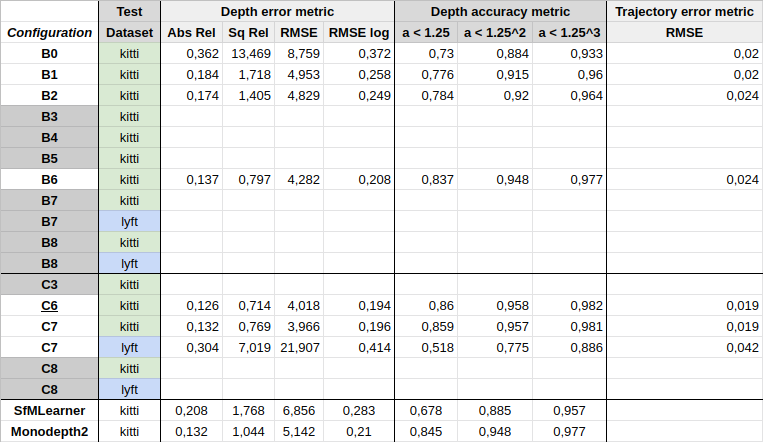
\includegraphics[width=1.0\textwidth]{evaluation}
	\caption{Evaluation metrics when testing the configurations on the testing split of the datasets}
	\label{fig:evaluation}
\end{figure}
\fi

\clearpage

\begin{figure}[H]
	\centering
	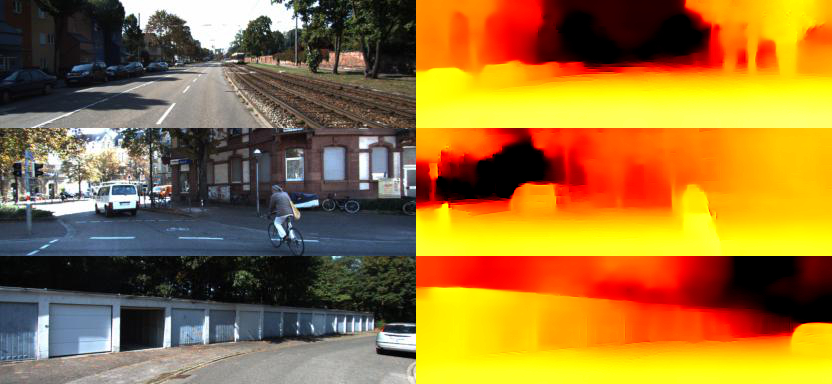
\includegraphics[width=1.0\textwidth]{depthmaps}
	\caption{Examples from the Kitti dataset}
	\label{fig:depthmapskitty}
\end{figure}

%\begin{figure}[H]
%	\centering
%	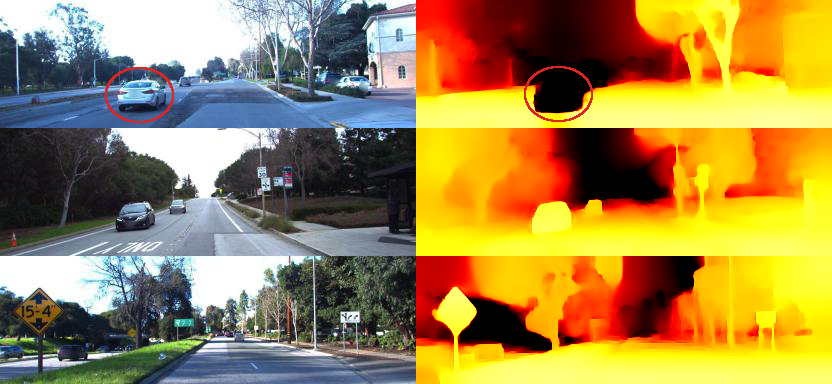
\includegraphics[width=1.0\textwidth]{depthmapslyft}
%	\caption{Examples from the Lyft dataset}
%	\label{fig:depthmaplyft}
%\end{figure}

\begin{figure}[H]
	\centering
	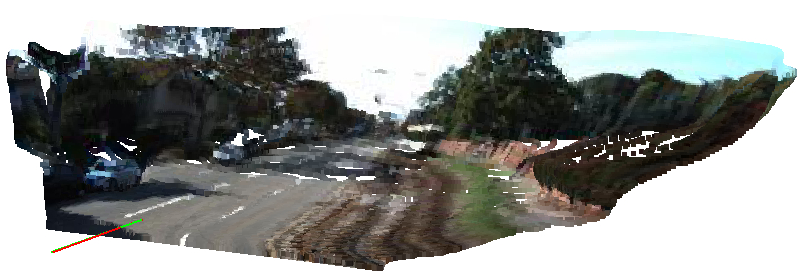
\includegraphics[width=0.8\textwidth]{3drender}
	\caption{3D render of colorized depth map}
	\label{fig:3drender}
\end{figure}

\begin{figure}[H]
	\centering
	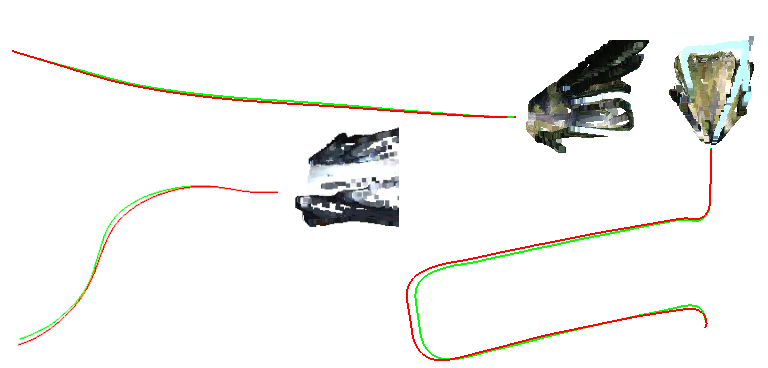
\includegraphics[width=0.8\textwidth]{motion2}
	\caption{3D visualization of the camera movement in three different image sequences. The green lines are the ground truth and the red lines are the predicted camera trajectories.}
	\label{fig:movement}
\end{figure}

\begin{figure}[H]
	\centering
	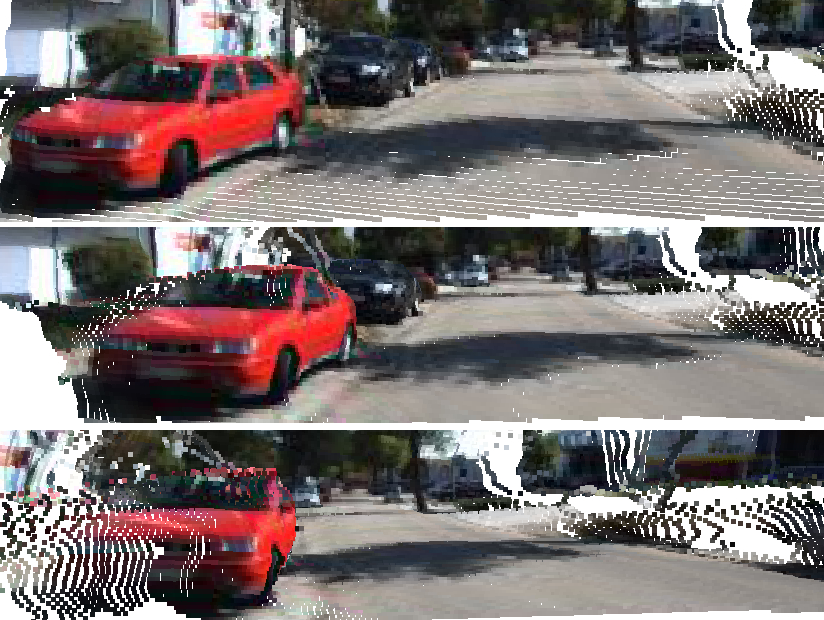
\includegraphics[width=0.8\textwidth]{3dseq}
	\caption{3D visualization from 3 different angles of the same frame in the kitti dataset.}
	\label{fig:3dseq}
\end{figure}

\section{Keypoint detection}

\begin{figure}[H]
	\centering
	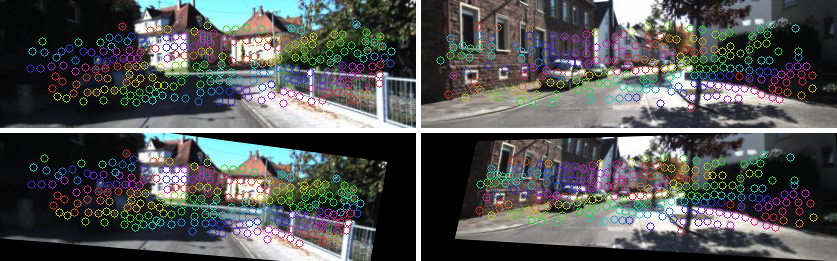
\includegraphics[width=1.0\textwidth]{point1}
	\caption{}
	\label{fig:point1}
\end{figure}

\begin{table}[H]
\centering
\begin{tabular}{|l|l|l|l|l|l|l|}
\hline
Method & RS $\uparrow$ & LE $\downarrow$ & MS $\uparrow$ & CMR $\uparrow$ & Nt & Nm \\
\hline
UnsuperPoint & 0.796 & \underline{0.666} & \underline{0.488} & \underline{0.834} & 338 & 203 \\
ORB & \underline{0.841} & 0.764 & 0.302 & 0.564 & 310 & 171 \\
\hline
\end{tabular}
\caption{Experiments measuring the performance of keypoint detection methods.}
\label{table:pointsbenchmark}
\end{table}

\section{Consensus maximization}

\begin{figure}[H]
	\centering
	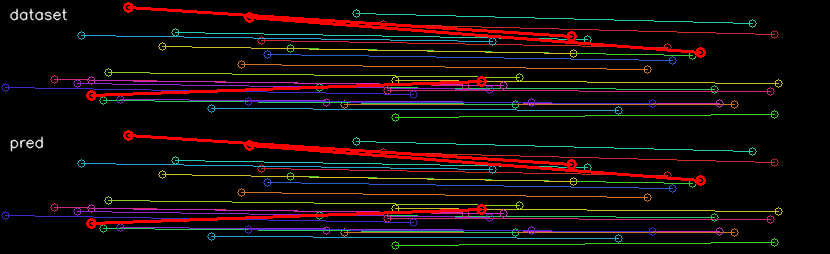
\includegraphics[width=1.0\textwidth]{synthhomo}
	\caption{Outlier detection in homography estimation in synthetic dataset. Top row is ground truth and bottom row is the prediction.}
	\label{fig:synthhomo}
\end{figure}

\begin{figure}[H]
	\centering
	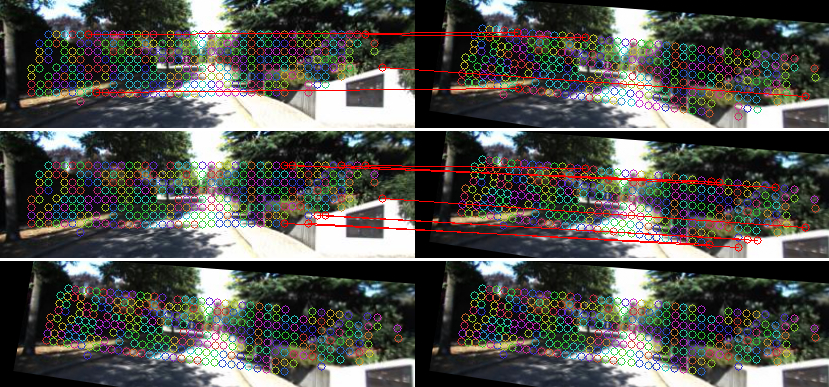
\includegraphics[width=1.0\textwidth]{kittihomo}
	\caption{Outlier detection and homography estimation on images from kitti dataset. First row is from OpenCV findHomography(), second row is from the network, third row is the image from branch A transformed by the homographgy found by OpenCV, fourth row is the image from branch A transformed by the homography found by the network.}
	\label{fig:kittihomo}
\end{figure}

\begin{table}[H]
	\centering
	\begin{tabular}{|l|l|l|l|}
		\hline
		Method & HE \\
		\hline
		ConsensusNet & ??? \\
		OpenCV RANSAC & ??? \\
		\hline
	\end{tabular}
	\caption{Metrics for homography estimation.}
	\label{table:pointsbenchmark}
\end{table}